\chapter{Multiple Alignment}
Until now we have discussed about alignment of a pair of sequences, and we have seen that for this problem we can find different algorithms for finding an optimal solution. But what for alignment of more than two sequences?
In this chapter we introduce a new idea of alignment that doesn't consider only an alignment between two sequences but among many of them. This kind of alignment is called \textbf{Multiple alignment}, it can reveal subtle similarities that pairwise alignment don't reveal.\\
Multiple sequence alignments are used for many reasons, including:
\begin{itemize}
	\item To detect regions of variability or conservation in a family of proteins.
	\item To provide stronger evidence than pairwise similarity for structural and functional inferences.
\end{itemize} 
\image{img/Multialignment}{Example of Multiple Alignment.}{0.9}
In order to better understand the concept of multiple alignment it is possible to consider the relations between a two sequences alignment and a three sequences alignment. Alignment of two sequences is represented as a 2-row matrix, instead we represent alignment of three sequences as a \textbf{3-row matrix}.
\image{img/3RowMatrix}{Example of Multiple Alignment.}{0.3}
The resulting score considers the composition of columns, the more conserved they are the better is the alignment. In other words, if some columns are composed only by gaps the resulting score will be lower.

\section{Aligning 3 sequences}
Alignment of $3$ sequences consists on a multiple alignment problem for $3$ sequences. The adopted strategy is similar to the solution provided for the alignment of $2$ sequences (2-D edit graph computed using dynamic programming). Now the edit graph has a 3-D shape, in which each axis represent a sequence of the problem, and the global alignment is obtained going from the source to sink.
\image{img/cube3d.png}{3-D graph for alignment of 3 sequences.}{0.5}
The edit distance definition is now defined:
\image{img/3dedit.png}{Dynamic programming score definition with 3 sequences/dimension.}{0.8}
where $\delta(x,y,z)$ is an entry in a $3D$ scoring matrix.\\
This solution has a important limit, the time complexity. In fact we can easily check that, considering 3 sequences of length $n$, we have a time complexity equals to $7n^3 \rightarrow O(n^3)$. In general we can write that considering $K$ sequences we have $(2^K-1)(n^K) \rightarrow O(2^Kn^K)$.\\
In other words dynamic programming for 2 sequences can be extended in the case of $K$ sequences but still it is impractical due to exponential computation time.\\

\section{Heuristic method for multiple alignment: MSA}
It seems that exact methods cannot be applied, due to their complexities. In general we have multiple sequences \textbf{heuristic methods} are used.
\textbf{MSA} is an heuristic procedure, and its main characteristic is that it induces to multiple pairwise alignments (PA). In other words every multiple alignment induces more pairwise ones.
\image{img/msa.png}{MSA pairwise alignment.}{0.8}
Once that the problem has been decomposed in multiple pairwise alignment it is necessary to reconstructing a multiple alignment starting from pairwise alignments. Given $K$ arbitrary pairwise alignment we cannot always construct a multiple alignment that induces them since PA may be inconsistent.

Consider the following examples:

\begin{figure}[h]
	\begin{minipage}[t]{0.5\linewidth}
		\centering
		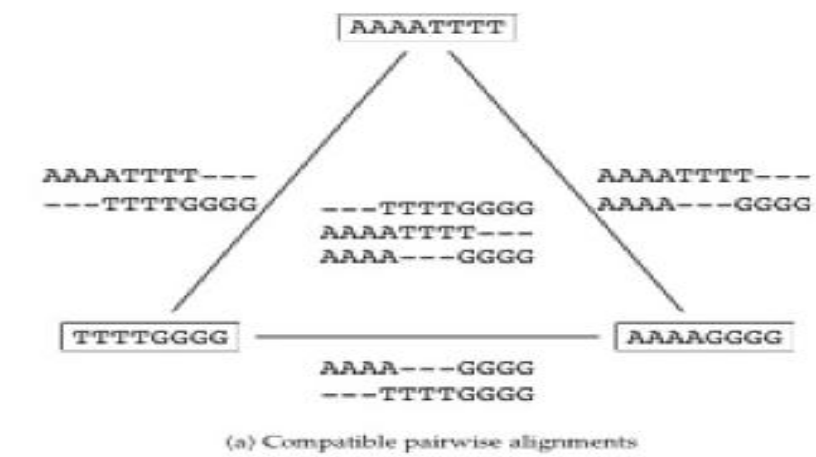
\includegraphics[width=1\textwidth]{img/simsa1.png}
		\caption{From optimal PAs to MSA.}
		\label{ex1PA}
	\end{minipage}
	\hspace{0.1cm}
	\begin{minipage}[t]{0.5\linewidth} 
		\centering
		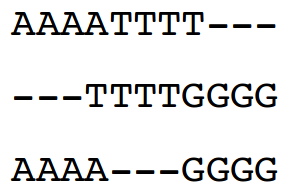
\includegraphics[width=1\textwidth]{img/simsa2.png}
		\caption{From optimal PAs to MSA.}
		\label{ex2PA}
	\end{minipage}        
\end{figure} 
 
Figures \ref{ex1PA} and \ref{ex2PA} show example of multiple pairwise alignments that can be combined into a single multiple-alignment, since there is no ambiguity. Instead if we consider the following example: \\

\begin{figure}[H]
	\begin{minipage}[t]{0.5\linewidth}
		\centering
		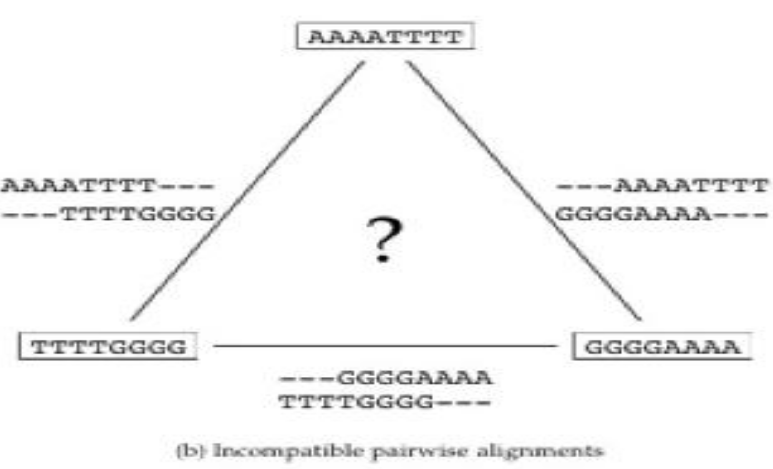
\includegraphics[width=1\textwidth]{img/nomsa1.png}
		\caption{From optimal PAs to MSA.}
		\label{ex3PA}
	\end{minipage}	
	\hspace{0.1cm}
	\begin{minipage}[t]{0.5\linewidth} 
		\centering
		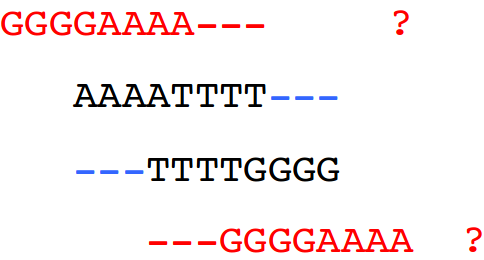
\includegraphics[width=1\textwidth]{img/nomsa2.png}
		\caption{From optimal PAs to MSA.}
		\label{ex4PA}
	\end{minipage}        
\end{figure} 
Figures \ref{ex3PA} and \ref{ex4PA} show an example of pairwise alignments that cannot be combined into a single multiple alignment since there is \textbf{ambiguity}. What we can see is that there is ambiguity because the sequence \verb|GGGGAAAA| can be either aligned on the A prefix or in the G suffix.\\

From an optimal multiple alignment we can infer pairwise alignments between all pairs of sequences, but they are not necessarily optimal. From optimal pairwise alignment between all pairs of sequences it is difficult to infer a \textbf{good multiple alignment}.
\section{Scores}
In order to get the best possible multiple alignment for MSA we introduce a score to each possible solution and we pick the best one. There exists 3 ways for computing the score:
\begin{itemize}
	\item Multiple Longest Common Subsequence score (LCS score)
	\item Entropy Score
	\item Sum of Pairs Score (SP score)
\end{itemize}
They have a common assumption: \textbf{Independence of positions.}


\paragraph{Multiple LCS score}
A column is a \textbf{match} if all the letters in the column are the same. The total score is the number of matches.
\image{img/lcs.png}{LCS Example.}{0.1}

This scoring algorithm is very good only for very similar sequences, and remember that still preserve the independence of positions.
\paragraph{Entropy score}
Define \textbf{frequencies} for the occurrence of each letter in each column of multiple alignment.

\begin{align}
\begin{bmatrix}
$A$&$A$&$A$ \\
$A$&$A$&$A$ \\
$A$&$A$&$T$ \\
$A$&$T$&$C$
\end{bmatrix}
\end{align}

\begin{itemize}
	\item $p_A = 1, p_T = p_G = p_C = 0$ ($1^{st}$ column)
	\item $p_A = 0.75, p_T = 0.25, p_G = p_C = 0$ ($2^{st}$ column)
	\item $p_A = 0.50, p_T = 0.25, p_G = 0.25, p_C = 0$ ($3^{st}$ column)
\end{itemize}
Compute \textbf{entropy} of each column:
$$- \sum_{X = A,T,G,C} p_x \times \log_2p_x$$
Example:
\begin{align}
entropy & \begin{bmatrix}
$A$ \\
$A$ \\
$A$ \\
$A$
\end{bmatrix} = 0 && \text{\textbf{Best case}}
\end{align}


\begin{align}
entropy & \begin{bmatrix}
$A$ \\
$T$ \\
$G$ \\
$C$
\end{bmatrix} = -\sum\frac{1}{4}\log_2\frac{1}{4} = 2 && \text{\textbf{Worst case}}
\end{align}
\textbf{Entropy for a multiple alignment} is the sum of entropies of its columns.
$$\sum_{\text{over all columns}}(- \sum_{X = A,T,G,C} p_x \times \log_2p_x)$$
Then the best alignment is reached minimizing this quantity.
\image{img/entropy.png}{Entropy score example.}{1}

\paragraph{Sum of Pairs} From a multiple alignment, we can infer pairwise alignments between all sequences, but they are not necessarily optimal. This is like projecting a 3D multiple alignment path onto a 2D face of the cube. In other words a 3D alignment can be projected onto a 2D plane to represent an alignment between a pair of sequences.
\image{img/projection3d.png}{All 3 Pairwise Projections of the Multiple Alignment}{0.4}

Consider pairwise alignment of sequences $a_i$ and $a_j$ imposed by a multiple alignment of $k$ sequences. Denote the score of this sub-optimal (not necessarily optimal) pairwise alignment as: $s^*(a_i,a_j)$. Sum up the pairwise score for a multiple alignment:
$$s(a_1,\dots,a_k) = \sum_{i,j} s^*(a_i,a_j) $$
It corresponds to consider more possible ancestors. In evolution, mutations are counted more than once. So, if we want to align $4$ sequences we have $6$ pairwise alignments.
Given $a_1$,$a_2$,$a_3$,$a_4$ we have:
$$s(a_1,\dots, a_4) = \sum s^*(a_i,a_j) = s^*(a_1,a_2)+s^*(a_1,a_3)+s^*(a_1,a_4)+s^*(a_2,a_3)+s^*(a_2,a_4)+s^*(a_3,a_4)$$
\image{img/sumpairsexample.png}{Sum of Pairs Score example.}{0.8}

\subsection{Representation of MSA: Profile}
\image{img/msaprofile.png}{MSA representation Example.}{0.8}
MSA representation takes in consideration:
\begin{itemize}
	\item Symbols frequencies
	\item It is an \textbf{exact and compact representation} of the multiple alignment
	\item A \textbf{threshold} can simplify the profile
	\item Useful for searching in DB
	\item We can align a sequence against a profile
	\item We can align a profile against a profile
\end{itemize}

\subsection{Aligning alignments}
Another interesting problem regards the possibility of aligning two different alignments.

\image{img/alignalignments.png}{Align alignments example.}{0.5}

A suggestion consists on considering the two profiles.

\subsection{Aligning a sequence to an alignment}
We define as $R_{ij}$ element of the score matrix (PAM/BLOSUM) and $x = x_1 \dots x_m$ sequence to be aligned. We want to align a profile $A$ with m columns.

\begin{align}
x_k \text{~is~aligned to}~~~ A_h = & \begin{bmatrix}
a_1 \\
\dots \\
a_n
\end{bmatrix}
\end{align}

\textbf{Score}(x,A) = $\sum_isc(x_i,A_i)\qquad i \in [1,m]$ with\\
\textbf{sc}($x_k, A_h$) = $\sum_ia_iR_{xki} \qquad i \in [1,21]$

\subsection{Aligning an alignment to an alignment}
We define $R_{ij}$ element of the score matrix (PAM/BLOSUM) and a profile $A$ to be aligned with another one $B$, both with m columns.

\begin{align}
B_h = & \begin{bmatrix}
b_1 \\
\dots \\
b_n
\end{bmatrix}
\end{align}

is aligned to:

\begin{align}
A_h = & \begin{bmatrix}
a_1 \\
\dots \\
a_n
\end{bmatrix}
\end{align}
\textbf{sc}$(A_h,B_k) = \sum_j\sum_ia_ib_jR_{ij} \qquad i,j \in [1,21]$\\
\textbf{score}$= \sum_k sc(A_k, B_k) \qquad k \in [1,m]$

\section{Heuristic Methods for MSA}
MSA can be solved by different heuristic methods:
\begin{itemize}
	\item Carillo-Lipman method
	\item Heuristic Greedy method
	\item Progressive Alignments (ClustalW)
	\item Iterative Alignments (Deterministic and Stochastic)
	\item Partial Order Alignments (POA)
\end{itemize}

\subsection{Carillo-Lipman}
One of the heuristic algorithms for MSA is the \textbf{Carillo-Lipman Bound procedure}(1988). It computes a polyhedron around the diagonal in a hypercube. This bounds the search space for finding MSA. It computes the optimal alignment scores only in the grey volume. 
\image{img/carillo.png}{Carillo-Lipman space.}{0.3}
The grey volume is computed on the one side by the optimal alignments found for each pair of sequences, and on the other by a heuristic multiple alignment of the 3 sequences.\\

\paragraph{Procedure.} The method can be easily described with the following steps:
\begin{itemize}
	\item Consider the pairwise alignments of each pair of sequences and create a phylogenetic tree from these scores.
	\item produce a draft MSA built from the phylogenetic tree.
	\item the pairwise alignments and draft MSA provide a \textbf{reduced solution space} on which dynamic programming is used to find the solution.
\end{itemize}

\paragraph{Properties.} This methods does not guarantee an optimal alignment for all the sequences because most of the solution space is excluded from search. It is useful when at most 8 sequences of average size and similarity need to be aligned.

\subsection{Heuristic Greedy Approach}
The algorithm works:\\ 
"\textit{Choose most similar pair of strings and combine them into a profile, thereby reducing alignment of k sequences to an alignment of $k-1$ sequences/profiles. Repeat.}"\\

This is a heuristic greedy method that can be applied both to sequences and to profiles.

\image{img/heuristicGreedy.png}{Heuristic Greedy Method.}{0.7}
Consider these $4$ sequences:
\image{img/heuristicExample.png}{Sequences Example.}{0.3}
with scores: match = 1, mismatch = -1 and gap = -1.

\image{img/heuristicSolvedExample.png}{Solution for heuristic example procedure(1).}{0.7}

\image{img/heuristicExampleSolved2.png}{Solution for heuristic example procedure(2).}{0.6}

\subsection{Progressive Alignments (ClustalW)}
Progressive alignment is a variation of the greedy algorithm with a somewhat more intelligent strategy for choosing the order of alignments. It is based on the idea of building a phylogenetic tree out of the sequences, the tree is used to decide which sequences are aligned first, because of their similarity. We can find different algorithms like: CLUSTAL, T-COFFEE.

\paragraph{ClustalW}
Popular MSA tool based on progressive alignment. $W$ stands for \textit{weighted} since different parts of alignment can be weighted differently. The weights may depend by the sequences relations or by being over or under-estimated: Three-step process:
\begin{enumerate}
	\item Construct pairwise alignments.
	\item Build guide tree.
	\item Progressive alignments guided by the tree.
\end{enumerate}
Different score matrices can be used depending on sequences relations. Gaps are permanent and it can use profiles to compare sequences.\\

Algorithm definition:
\begin{enumerate}
	\item Align each sequence $v_i$ against each other $v_j$ giving a \textbf{similarity matrix}. Similarity is measured counting the ration between exact matches and sequence length. $$\text{similarity} = \frac{\text{exact matches}}{\text{sequence length}}$$ 
	\image{img/step1.png}{ClustalW step 1.}{0.5}
	
	\item Create \textbf{guide tree}, which roughly reflect evolutionary relations, using the similarity matrix. ClustalW uses the neighbor-joining method.
	\image{img/step2.png}{ClustalW step 2.}{0.5}
	
	\item Start by aligning two most similar sequences. Following the guide tree, add the next sequences, aligning them to the existing alignment.
	\image{img/step3.png}{ClustalW step 3.}{0.7}
	\image{img/step3_2.png}{ClustalW step 3 example.}{0.9}
	\begin{itemize}
		\item \textbf{*} identical.
		\item \textbf{:} conserved substitution (same group).
		\item \textbf{.} semi-conserved subdivision (similar shapes).
	\end{itemize}
\end{enumerate}

\paragraph{Properties}
Progressive alignment is the most widely used method. It has some advantages:
\begin{itemize}
	\item \textbf{Speed}
	\item \textbf{Simplicity}
	\item A reasonable \textbf{Sensitivity}
\end{itemize}
But it has also some disadvantages:
\begin{itemize}
	\item It is an \textbf{heuristic method}
	\item It is \textbf{highly sensitive} to the choice of initial aligned pairs
	\item The initial pairs are \textbf{frozen} even if subsequent steps show that they are not correct
	\item The likelihood of large errors in the initial alignments increases as the sequences become more distantly related, hence they work well for close sequences, but they \textbf{deteriorate for distance sequences}.
\end{itemize}

\subsection{Iterative Alignments - Deterministic}
Progressive alignment results can be sensitive to inaccuracies in the initial pairwise alignments. Iterative methods produce an initial global alignment (i.e. obtained by a progressive method) and then iteratively refine it in order to \textbf{optimize an objective function}. The algorithm works as follow:
\image{img/iterative.png}{Iterative alignments procedure.}{1}
The procedure is guaranteed to \textbf{converge to a local maximum}. If the initial alignment is poor, it may not converge to the global maximum. Examples of deterministic iterative approaches are: PRRP, DIALIGN, etc...

\subsection{Iterative Alignments - Stochastic}
\begin{itemize}
	\item \textbf{Genetic Algorithm:}
	\begin{itemize}
		\item Randomly generate MSA (generations)
		\item Alignments die or survive depending on their fitness (score)
		\item Mutations rearrange them with the introduction of gaps at varying positions or recombine them.	
		\item An objective function is optimized.
	\end{itemize} 

	\item \textbf{Simulated Annealing:}
	\begin{itemize}
		\item An alignment is randomly modified
		\item Its score is assessed
		\item according to an acceptance function it is kept or discarted.
		\item The acceptance function becomes more stringent at each iteration.
	\end{itemize} 
	\item \textbf{Hidden Markov Models}
	\item \textbf{Not ab initio!}
\end{itemize}

\subsection{Partial Order Multiple Alignment (POA)}
Multidomain proteins evolve not only through point mutations but also though \textbf{domain duplications} and \textbf{domain re-combinations}. Often impossible to align all protein sequences throughout their entire length.
\image{img/alignmedGraph.png}{Alignmed as a Graph.}{0.95}
\image{img/pathgraph.png}{Representing sequences as paths in a graph.}{0.95}

Partial Order Multiple Alignment has two goals:
\begin{itemize}
	\item Finding a graph that represents a domain structure (model).
	\item Finding mapping of each sequence to this graph.
\end{itemize}
The solution consists on using the PO-MSA algorithm, which basically construct a graph G such that every sequence in the set of sequences S is a path in G. \\
The POA algorithm aligns sequences onto a directed acyclic graph (DAG):
\begin{itemize}
	\item Guide Tree Construction
	\item Progressive Alignment Following Guide Tree
	\item Dynamic Programming Algorithm to align two PO-MSAs (PO-PO Alignment).
\end{itemize}
Alignments of graphs is done using the dynamic programming definition:

$$S(n,o) = \text{max}_{p\rightarrow n, q \rightarrow o} \begin{cases}
S(p,q) + s(n,o) & \\
S(p,o) + \Delta(n) & \text{n: node in G}\\
S(n,q) + \Delta(o) & \text{o: node in G}^\prime
\end{cases}$$
Then value $S(n,o)$ represents the score assigned to the alignment, with $s(n,o)$ as the cost of match or mismatch between node n and o, and with $\Delta(n)$, $\Delta(o)$ as the costs for deleting node n or node o from the alignment.

\section{Multiple Alignments Remarks}
For MSA there is no satisfactory theory, improvements driven by results, not by the theory. For that reason importance of visualization tools can be important for the evaluation and inspection. In particular we have two types of representations:
\begin{itemize}
	\item \textbf{Visualization (ClustalX)} 
	\image{img/clustalx.png}{Visualization of MSA.}{0.85}
	
	\item \textbf{Visualization: sequence logo}
	\image{img/logo.png}{Visualization: sequence logo}{0.8}
	 A sequence logo shows the more conserved residues as larger characters, the total height of a column is proportional to how conserved that position is.

\end{itemize}
